\documentclass[english, 12pt]{article}
\usepackage{enumerate}
\usepackage{fancyhdr}
\usepackage{pgfplots}
\pgfplotsset{width=10cm,compat=1.9}

% We will externalize the figures
\usepgfplotslibrary{external}
\tikzexternalize

\begin{document}

\title{COP290 Lab 2}

\author{
  Anish Banerjee  \and
  Aman Singh Dalawat \and
  Jay Patel 
}
% \date{xx/xx/xx} %uncomment this to place a specific date or leave it blank to erase the date 

\maketitle

\section{Introduction}\label{introduction}
In this report, we perform a comparative analysis of concurrency and parallelism. \textbf{Concurrency} refers to the ability of a computer system to execute multiple tasks using shared resources in such a way that at a given instant of time only one task is running. \textbf{Parallelism} is the ability to execute multiple tasks or processes at the same time using multiple processors or cores.
 


\section{Comparative Analysis}
To time the files, we have used the \textit{time} command on the shell. It provides us with three metrics
\begin{enumerate}
\item{\textbf{real} is wall clock time - time from start to finish of the call.}
\item{\textbf{user} is the amount of CPU time spent in executing code that is written in the program itself.}
\item{\textbf{sys} is the amount of CPU time spent in executing operating system functions on behalf of the program. }
\end{enumerate}

Thus, in our analysis, we use real times to compare concurrency with parallelism.

\subsection{Number of Files V/s Time}

\begin{center}
\begin{tabular}{|c|c|c|}
\hline
Number of files &
  Time(Concurrency) &
  Time(Paralellism) \\
\hline
1 &
  \begin{tabular}[c]{@{}l@{}}real 2.968s\\ user 2.644s\\ sys 0.324s\end{tabular} &
  \begin{tabular}[c]{@{}l@{}}real 3.926s\\ user 3.516s\\ sys 0.410s\end{tabular} \\
\hline
3 &
  \begin{tabular}[c]{@{}l@{}}real 8.882s\\ user 7.885s\\ sys 0.996s\end{tabular} &
  \begin{tabular}[c]{@{}l@{}}real 6.452s\\ user 14.899s\\ sys 2.018s\end{tabular} \\
\hline
6 &
  \begin{tabular}[c]{@{}l@{}}real 17.929s\\ user 15.841s\\ sys 2.068s\end{tabular} &
  \begin{tabular}[c]{@{}l@{}}real 8.195s\\ user 33.042s\\ sys 7.040s\end{tabular} \\
\hline
8 &
  \begin{tabular}[c]{@{}l@{}}real 23.730s\\ user 21.224s\\ sys 2.504s\end{tabular} &
  \begin{tabular}[c]{@{}l@{}}real 10.037\\ user 48.944s\\ sys 12.401s\end{tabular} \\
\hline
10 &
  \begin{tabular}[c]{@{}l@{}}real 29.937s\\ user 26.450s\\ sys 3.427s\end{tabular} &
  \begin{tabular}[c]{@{}l@{}}real 12.729s\\ user 1m 9.223s\\ sys 21.343s\end{tabular}\\
\hline
\end{tabular}\\ 
\vspace{5pt}
\caption{Table 2.1: Here files with 1 million lines (70mB) each are used}
\label{tab: Table 2.1}

\vspace{10pt}
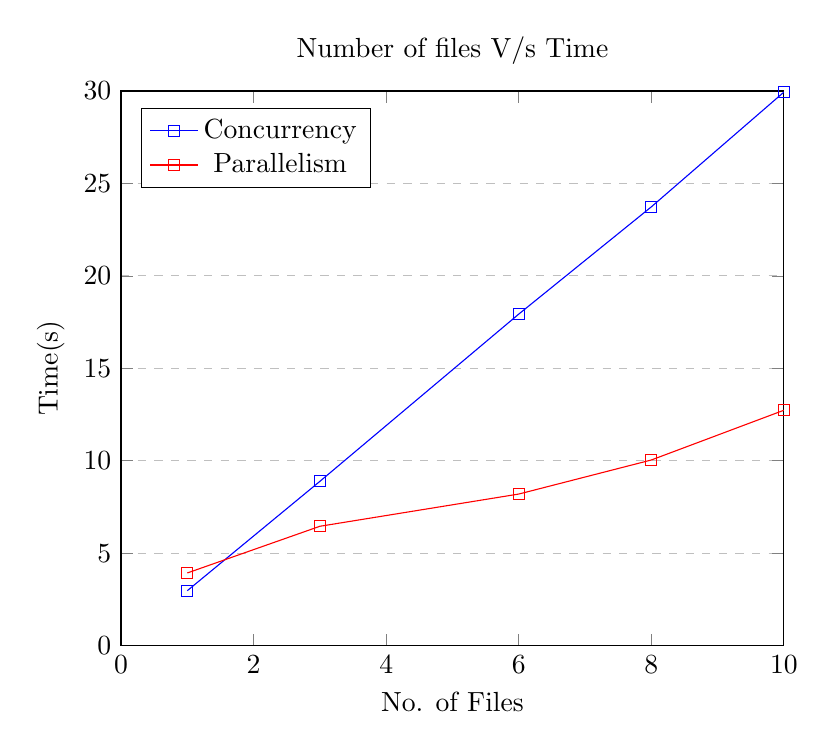
\begin{tikzpicture}
\begin{axis}[
    title={Number of files V/s Time},
    xlabel={No. of Files },
    ylabel={Time(s)},
    xmin=0, xmax=10,
    ymin=0, ymax=30,
    xtick={0,2,4,6,8,10},
    ytick={0,5,10,15,20,25,30},
    legend pos=north west,
    ymajorgrids=true,
    grid style=dashed,
]

\addplot[
    color=blue,
    mark=square,
    ]
    coordinates {
    (1,2.968)(3,8.882)(6,17.929)(8,23.730)(10,29.937)
    };

 \addplot[
    color=red,
    mark=square,
    ]
    coordinates {
    (1,3.926)(3,6.452)(6,8.195)(8,10.037)(10,12.729)
    };
    \legend{Concurrency,Parallelism}   
\end{axis}
\end{tikzpicture}
\end{center}

\subsection{Same Word Repeated Multiple Times V/s Time}

\begin{center}
\begin{tabular}{|c|c|c|}
\hline
Number of files &
  Time(Concurrency) &
  Time(Parallelism) \\
  \hline
1 &
  \begin{tabular}[c]{@{}l@{}}real 0.454s\\ user 0.405s\\ sys0.048s\end{tabular} &
  \begin{tabular}[c]{@{}l@{}}real 0.761s\\ user 0.651s\\ sys0.082s\end{tabular} \\
  \hline
3 &
  \begin{tabular}[c]{@{}l@{}}real 1.344s\\ user 1.220s\\ sys 0.124s\end{tabular} &
  \begin{tabular}[c]{@{}l@{}}real 2.807s\\ user 2.595s\\ sys 1.991s\end{tabular} \\
  \hline
6 &
  \begin{tabular}[c]{@{}l@{}}real 2.701s\\ user 2.420s\\ sys 0.281s\end{tabular} &
  \begin{tabular}[c]{@{}l@{}}real 7.596s\\ user 8.119s\\ sys 11.310s\end{tabular} \\
  \hline
8 &
  \begin{tabular}[c]{@{}l@{}}real 3.595s\\ user 3.215s\\ sys 0.380s\end{tabular} &
  \begin{tabular}[c]{@{}l@{}}real 11.019s\\ user 12.691s\\ sys 21.746s\end{tabular} \\
  \hline
10 &
  \begin{tabular}[c]{@{}l@{}}real 4.497s\\ user 4.085s\\ sys 0.412s\end{tabular} &
  \begin{tabular}[c]{@{}l@{}}real 14.974s\\ user 17.555s\\ sys 35.812s\end{tabular}\\
  \hline
\end{tabular}
\vspace{5pt} \\
\caption{Table 2.2:Here the same word "hello" repeated 2 million times}
\label{tab:Table 2.2}
\vspace{12pt}
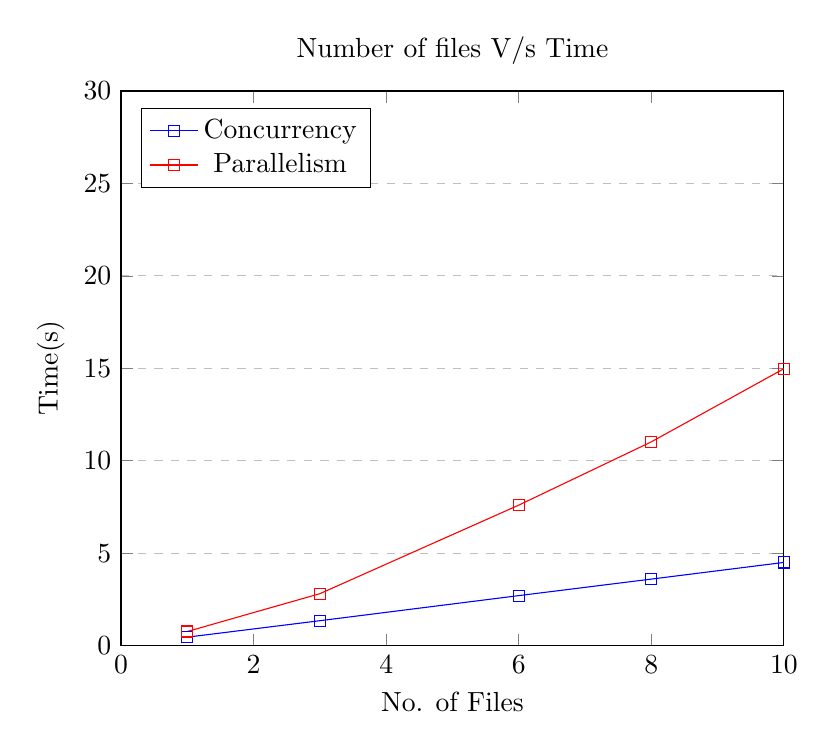
\begin{tikzpicture}
\begin{axis}[
    title={Number of files V/s Time},
    xlabel={No. of Files },
    ylabel={Time(s)},
    xmin=0, xmax=10,
    ymin=0, ymax=30,
    xtick={0,2,4,6,8,10},
    ytick={0,5,10,15,20,25,30},
    legend pos=north west,
    ymajorgrids=true,
    grid style=dashed,
]

\addplot[
    color=blue,
    mark=square,
    ]
    coordinates {
    (1,0.454)(3,1.344)(6,2.701)(8,3.595)(10,4.497)
    };

 \addplot[
    color=red,
    mark=square,
    ]
    coordinates {
    (1,0.761)(3,2.807)(6,7.596)(8,11.019)(10,14.974)
    };
    \legend{Concurrency,Parallelism}   
\end{axis}
\end{tikzpicture}
\end{center}

\subsection{Size of Files V/s Time}

\begin{center}
\begin{tabular}{|c|c|c|}
\hline
Size of file &
Time(Concurrency) &
Time(Parallelism)\\ \hline
10mB &
  \begin{tabular}[c]{@{}l@{}}real 0.981s\\ user 0.791s\\ sys 0.072s\end{tabular} &
  \begin{tabular}[c]{@{}l@{}}real 1.068s\\ user 0.942s\\ sys 0.112s\end{tabular} \\ \hline
20mB &
  \begin{tabular}[c]{@{}l@{}}real 1.729s\\ user 1.519s\\ sys 0.157s\end{tabular} &
  \begin{tabular}[c]{@{}l@{}}real 2.052s\\ user 1.832s\\ sys 0.171s\end{tabular} \\ \hline
40mB &
  \begin{tabular}[c]{@{}l@{}}real 3.318s\\ user 3.106s\\ sys 0.201s\end{tabular} &
  \begin{tabular}[c]{@{}l@{}}real 3.890s\\ user 3.493s\\ sys 0.371s\end{tabular} \\ \hline
60mB &
  \begin{tabular}[c]{@{}l@{}}real 5.020s\\ user 4.689s\\ sys 0.305s\end{tabular} &
  \begin{tabular}[c]{@{}l@{}}real 5.699s\\ user 5.244s\\ sys 0.428s\end{tabular} \\ \hline
100mB &
  \begin{tabular}[c]{@{}l@{}}real 8.050s\\ user 7.491s\\ sys 0.548s\end{tabular} &
  \begin{tabular}[c]{@{}l@{}}real 9.361s\\ user 8.654s\\ sys 0.636s\end{tabular} \\ \hline

\end{tabular} \\ 
\vspace{5pt}

\label{tab:Table2.3}
\caption{Table 2.3: Size of files V/s Time}
\vspace{12pt}
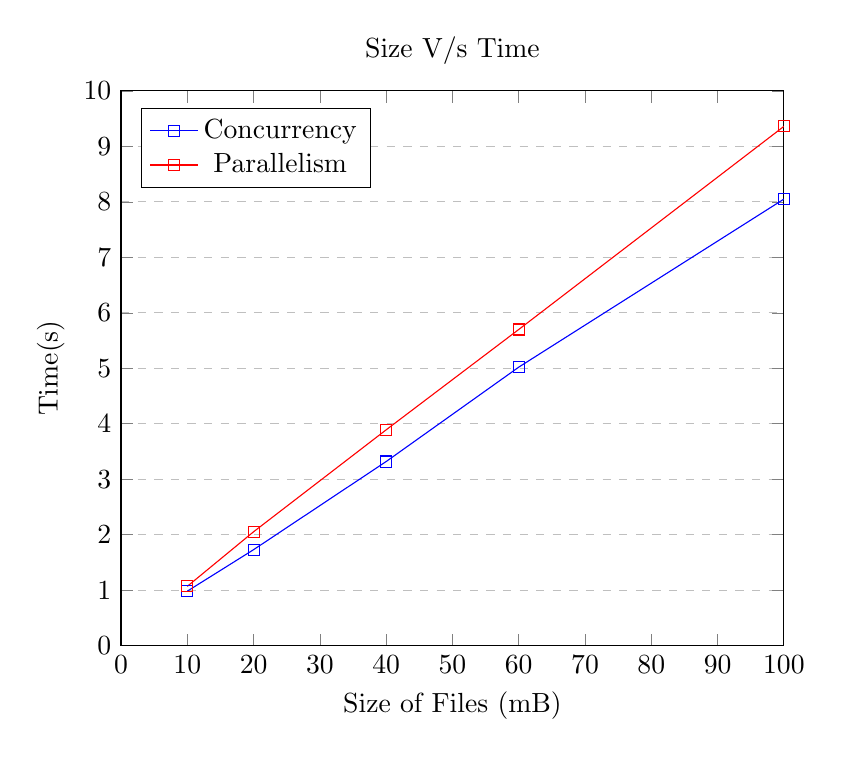
\begin{tikzpicture}
\begin{axis}[
    title={Size V/s Time},
    xlabel={Size of Files (mB) },
    ylabel={Time(s)},
    xmin=0, xmax=100,
    ymin=0, ymax=10,
    xtick={0,10,20,30,40,50,60,70,80,90,100},
    ytick={0,1,2,3,4,5,6,7,8,9,10},
    legend pos=north west,
    ymajorgrids=true,
    grid style=dashed,
]

\addplot[
    color=blue,
    mark=square,
    ]
    coordinates {
    (10,0.981)(20,1.729)(40,3.318)(60,5.020)(100,8.050)
    };

 \addplot[
    color=red,
    mark=square,
    ]
    coordinates {
    (10,1.068)(20,2.052)(40,3.890)(60,5.699)(100,9.361)
    };
    \legend{Concurrency,Parallelism}   
\end{axis}
\end{tikzpicture}
\end{center}
\textbf{System Specification used to run above files:}\\
Processor: Ryzen 7 5700U 8 cores \\
RAM: 16GB DDR4
\section{Observations}
\begin{itemize}
    \item In case 2.1, parallelism takes much less time as compared to concurrency as the number of files increases
    \item In case 2.2, parallelism takes more time than concurrency as the file size increases
    \item In case 2.3, parallelism and concurrency take almost same time (though, concurrency is slightly better)
\end{itemize}

\section{Why are the Differences Observed?}
\begin{itemize}
    \item \textbf{Case 2.1} :In concurrency, we are running files with the help of multiple threads but at a given time only one of the threads is working and reading a specific file. In parallelism, we have multiple threads running on multiple files, and at a given instant multiple files can run, so the overall time when running more than one file can be seen to be a lot less. In the case of only one file running we see there is not much difference in the running time because at a given instant only a single file is running in both implementations.
    \item \textbf{Case 2.2}:In this case we see the code with concurrency runs considerably faster than the parallelism-based code, even on multiple files. This is because of the implementation of locks in the case of parallelism. Since many files are being read using multiple threads at the same time, all of them try to increment the count in the bucket of the same word, resulting in contention. Hence at a given instant only one of them is able to actually increment the word in the bucket. This defeats the whole purpose of running multiple files at the same time as the actual work is done only for one file at a time. Hence in this case, parallelism-based implementation falls behind concurrency-based implementation by a larger margin because of the complexity of repeated acquisition and release of locks.
    \item \textbf{Case 2.3}:In the case of a single file running, where the task is not necessarily computationally intensive, concurrency slightly outperforms the approach of parallelism because the overhead of managing multiple threads or processes outweighs the performance gains achieved by the parallelism approach. Additionally, parallelism may not be useful if the task is not divisible into smaller sub-tasks.
\end{itemize}

\section{Conclusion}
Thus, we conclude that both concurrency and parallelism have their own advantages and disadvantages. In the case of running several files with dissimilar words, it is better to use parallelism, whereas while handling similar words, it is better to use concurrency.

\section{Questions in Part 2 Checkpoint 3}
\subsection{Does the output vary?}
Yes, the output is lesser than the one obtained while running without mythread\_yield().
\subsection{Why do you think the output varies?}
The output varies because of the \textbf{race conditions} created due to the swapping of contexts in mythread\_yield(). When we are running mythread\_yield on a given word, say \textit{hello}, the execution of the context is paused. Assume that the initial count of \textit{hello} is 5. Then its value is not updated to 6 before swapping the context. Now when a new context encounters \textit{hello}, then it reads its count as 5 and not 6. So it will update the value as 6 when the context returns, resulting in lesser counts. This problem can be solved by the use of locks.


\section*{Group Work Assessment}


\begin{center}
\begin{tabular}{|c|c|c|}
\hline
Name & Number of Tokens & Work done \\ \hline
\begin{tabular}[c]{@{}l@{}}Aman Singh Dalawat\\ (2021CS50610)\end{tabular} & 10/30 & Hashmap, Comparative analysis\\
\hline
\begin{tabular}[c]{@{}l@{}}Anish Banerjee\\ (2021CS10134)\end{tabular}     & 10/30            & Part1, mythread\_yield, locks, \LaTeX  report \\
\hline
\begin{tabular}[c]{@{}l@{}}Jay Patel\\ (2021CS50617)\end{tabular} &
  10/30 &
  \begin{tabular}[c]{@{}l@{}}Linked list, mythread\_create, mythread\_join, \\ Documentation using Doxygen\end{tabular}\\
  \hline
\end{tabular}
\end{center}
\end{document}